% Figure: diamond inheritance with checkable joins (story 2).
% Build: pdflatex diamond_inheritance.tex  (run inside figures/)
\documentclass[tikz,border=6pt]{standalone}
\usetikzlibrary{positioning,arrows.meta}
\begin{document}
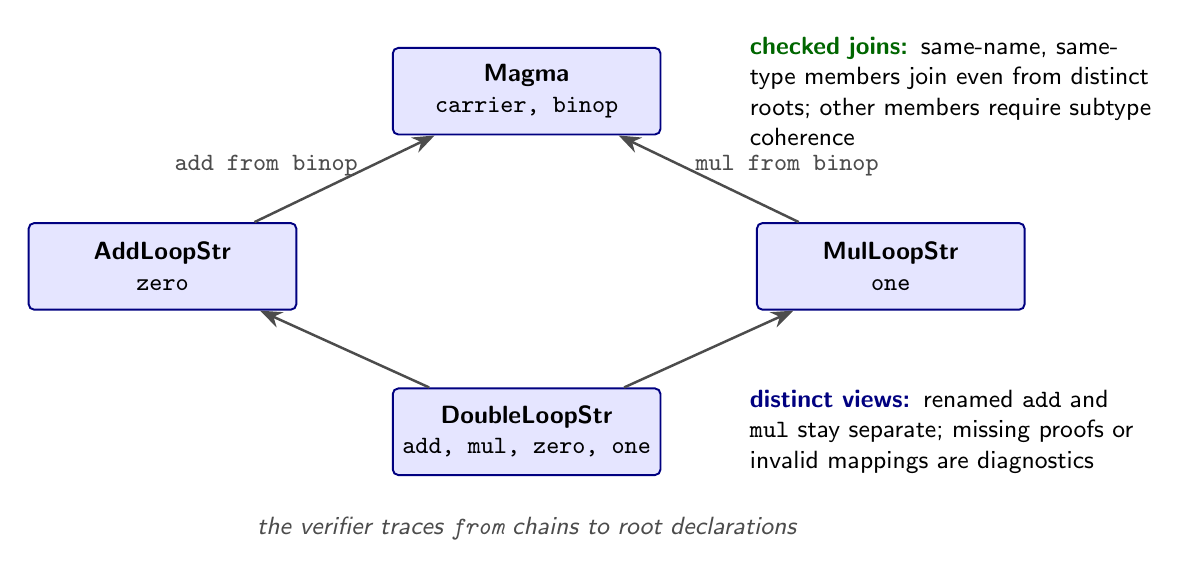
\begin{tikzpicture}[
  font=\sffamily,
  struct/.style={draw, rounded corners=2pt, align=center, minimum width=34mm,
                 minimum height=11mm, line width=0.7pt, fill=blue!10,
                 draw=blue!50!black, font=\sffamily\small},
  inh/.style={-{Stealth[length=2.8mm]}, line width=0.9pt, black!70},
  map/.style={font=\sffamily\small\ttfamily, text=black!70, align=center},
  check/.style={font=\sffamily\small, align=left},
]
  \node[struct] (magma) {\textbf{Magma}\\ \texttt{carrier, binop}};
  \node[struct, below left=11mm and 12mm of magma] (add)
    {\textbf{AddLoopStr}\\ \texttt{zero}};
  \node[struct, below right=11mm and 12mm of magma] (mul)
    {\textbf{MulLoopStr}\\ \texttt{one}};
  \node[struct, below=32mm of magma] (dbl)
    {\textbf{DoubleLoopStr}\\ \texttt{add, mul, zero, one}};

  \draw[inh] (add) -- node[map, above left=-1mm and -3mm] {add from binop} (magma);
  \draw[inh] (mul) -- node[map, above right=-1mm and -3mm] {mul from binop} (magma);
  \draw[inh] (dbl) -- (add);
  \draw[inh] (dbl) -- (mul);

  \node[check, right=10mm of magma, align=left, text width=52mm]
    {\textcolor{green!40!black}{\textbf{checked joins:}} same-name,
     same-type members join even from distinct roots; other members require
     subtype coherence};
  \node[check, right=10mm of dbl, align=left, text width=52mm]
    {\textcolor{blue!50!black}{\textbf{distinct views:}} renamed \texttt{add}
     and \texttt{mul} stay separate; missing proofs or invalid mappings are
     diagnostics};

  \node[font=\sffamily\small\itshape, text=black!70, below=4mm of dbl]
    {the verifier traces \texttt{from} chains to root declarations};
\end{tikzpicture}
\end{document}
